\chapter{Cybersecurity and Society}
\cite{04_Sociology} - 20hrs module\\
Objectives of this module:
\begin{itemize}
    \item Gain an introduction to sociology, its terminology, relevant theories, and risk sociology applicable to Cybersecurity.
    \item Understand the fundamental concepts of cybercrime and cybersecurity from a sociotechnical perspective.
    \item Explore the social, cultural, and organizational dimensions of cybercrime.
    \item Develop skills in identifying, analyzing, and mitagating cyber threats with a focus on social impacts.
\end{itemize}
It is relevant to learn more about cybersecurity in the societal sphere because "Humans are authors within Society".
\section{Sociology, Really?}
\subsection{What is Sociology?}
Some definitions to sociology.

\begin{displayquote}
    The science of social phenomena subject to natural and invariable laws, with goal of discovering these laws.
\end{displayquote}
\hfill -- Auguste Comte 
\newline

This assertion is overly positivist, as it overlooks potential negative impacts and seems somewhat naive. There are no general laws that describe social phenomena. In the modern view, in fact, no laws exist a priori. Some key parameters in Sociology: historical context and humankind.

\begin{displayquote}
    Sociology is the study of human social life, groups and societies.
\end{displayquote}
\hfill -- Sir Anthony Giddens

A post-positivist claim, states that there are no strong natural laws. This perspective is much more dynamic and mechanistic.

\begin{displayquote}
    Sociology is the scientific study of society, including the intricate patterns of \textbf{social behavior, relationships and human interactions}. It is a systematic examination of social institutions, \textbf{cultural norm} and social change, \textbf{using empirical research and critical analysis}. This discipline aims to understand the underlying mechanisms that govern \underline{social order}, dynamics and transformation, ranging from \textbf{individual interactions at the micro level} to \textbf{social structures at the macro level}. 
    Those in sociology investigate various aspects of human life, including social stratification, movement and change, with an emphasis on \textbf{how collective and individual behavior shapes and is shaped} by the broader social context.
\end{displayquote}
\hfill -- ChatGpt

\subsection{Ethics and Epistemic}

The main skill to develop is \textit{evaluative reasoning}, also referred to as *avalutativity*. This involves the ability to \textbf{assess, critique, and reflect on knowledge claims, methodologies, and ethical implications} in various contexts. In both ethical theory and epistemology\footnote{Epistemology is the branch of philosophy that studies the nature, scope, and limits of knowledge. }, individuals must be able to differentiate between valid and invalid arguments, recognize biases, and consider the consequences of knowledge application. The epistemic status of data is uncertain information (probabilistic way).
Other skills concern:
\begin{itemize}
    \item Extensivity: generalizing (macro), stimulus invariance, quantification
    \item Intensivity: understanding (micro), meaning to actions, qualification
\end{itemize}

\hfill -- Max Weber \footnote{European sociologist. 1864-1920.}

\subsection{Sociological Imagination}

Sociology offers explanations of social phenomena that are less biased than common sens and empirically grounded. Is a creative gift of the intellect that must be trained. In order to do that, Mills uses the idea of adopting a “Martian” perspective to encourage readers or philosophers to take an objective or detached view of societal norms. Observe micro- and macro-social phenomena without awe and wonder even if they are distant from us and seemingly disconnected. Not taking everyday life and what is *normal* (i.e. institutionalized) and (apparently) related to us for granted.

\hfill -- Charles W. Mills \footnote{American sociologist. 1916-1962.}

\begin{quote}
    You must train yourself to acquire new skills (a new normality) and avoid focusing on what feels strange. Instead, try to learn more from the other perspective.
\end{quote}

\subsection{Basic Sociological Vocabulary}
Keywords that unlock access to the cybercrime field from a sociological perspective.
\begin{itemize}
    \item Norms, i.e. rules and expectations that guide the behavior of members within a society. Cultures and languages also evolve according to certain norms. We can distinguish between two different types of norms:
    \begin{itemize}
        \item Silent norms: we adhere to them without the need to read them or be exposed to any formal institution. Most of these are acquired through imitation from families, social groups, etc.
        \item Codified norms: rules that are formally written down and established by an authoritative body, such as laws, regulations, or official guidelines.
    \end{itemize}
    \item Values: collective ideas about what is good, desirable, and proper.
        \begin{quote}
            A lighthouse in the darkness. 
        \end{quote}
    \item Role: set of norms, behaviors and expectations that are associated with a particular social status or position within a society. Roles guide how individuals are supposed to act and interact with others in specific contexts.
    \item Social structure: the organized pattern of social relationships and social institutions that together constitute society.
    \item Culture: shared beliefs, values and practices.
\end{itemize} \textbf{Insight on Role:}

It is possible to draw a dependency chain between: 
\begin{center}
    $\boxed{ \textcolor{blue}{Network}} \rightarrow \boxed{\textcolor{blue}{Position}} \rightarrow \boxed{\textcolor{blue}{Role}}$
\end{center}

In this chain, the Network represents the broader system of connections or relationships, which influences an individual’s Position within the structure. This position, in turn, determines the Role that the individual is expected to perform within the network. The interaction between these three elements highlights how individual behaviors and responsibilities are shaped by both social connections and hierarchical placement.

\begin{displayquote}
    You can do it without an actor, but it is the role that carries all the expectations.
\end{displayquote}

\subsection{Cybersecurity and Society}

The figure \ref{fig:Sociology_Iceberg} depicts the “Iceberg Model” of Sociology, which illustrates the visible and invisible elements that influence social dynamics. Similarly, in cybersecurity, there are layers of visible actions and hidden processes that determine the behavior and vulnerabilities of systems.
There are relationships between perceptions (what I see) and behaviors (how you act). Social interactions are also crucial, in fact, as they form the vast ocean of sociological imagination. Sociological imagination pertains to primary and secondary socialization. Primary socialization refers to the process by which individuals, typically in early childhood, learn and internalize the norms, values, beliefs, and behaviors of their culture or society, while secondary socialization develops when individuals step outside their comfort zone, though begins even before we are born.

\begin{figure}[H]
    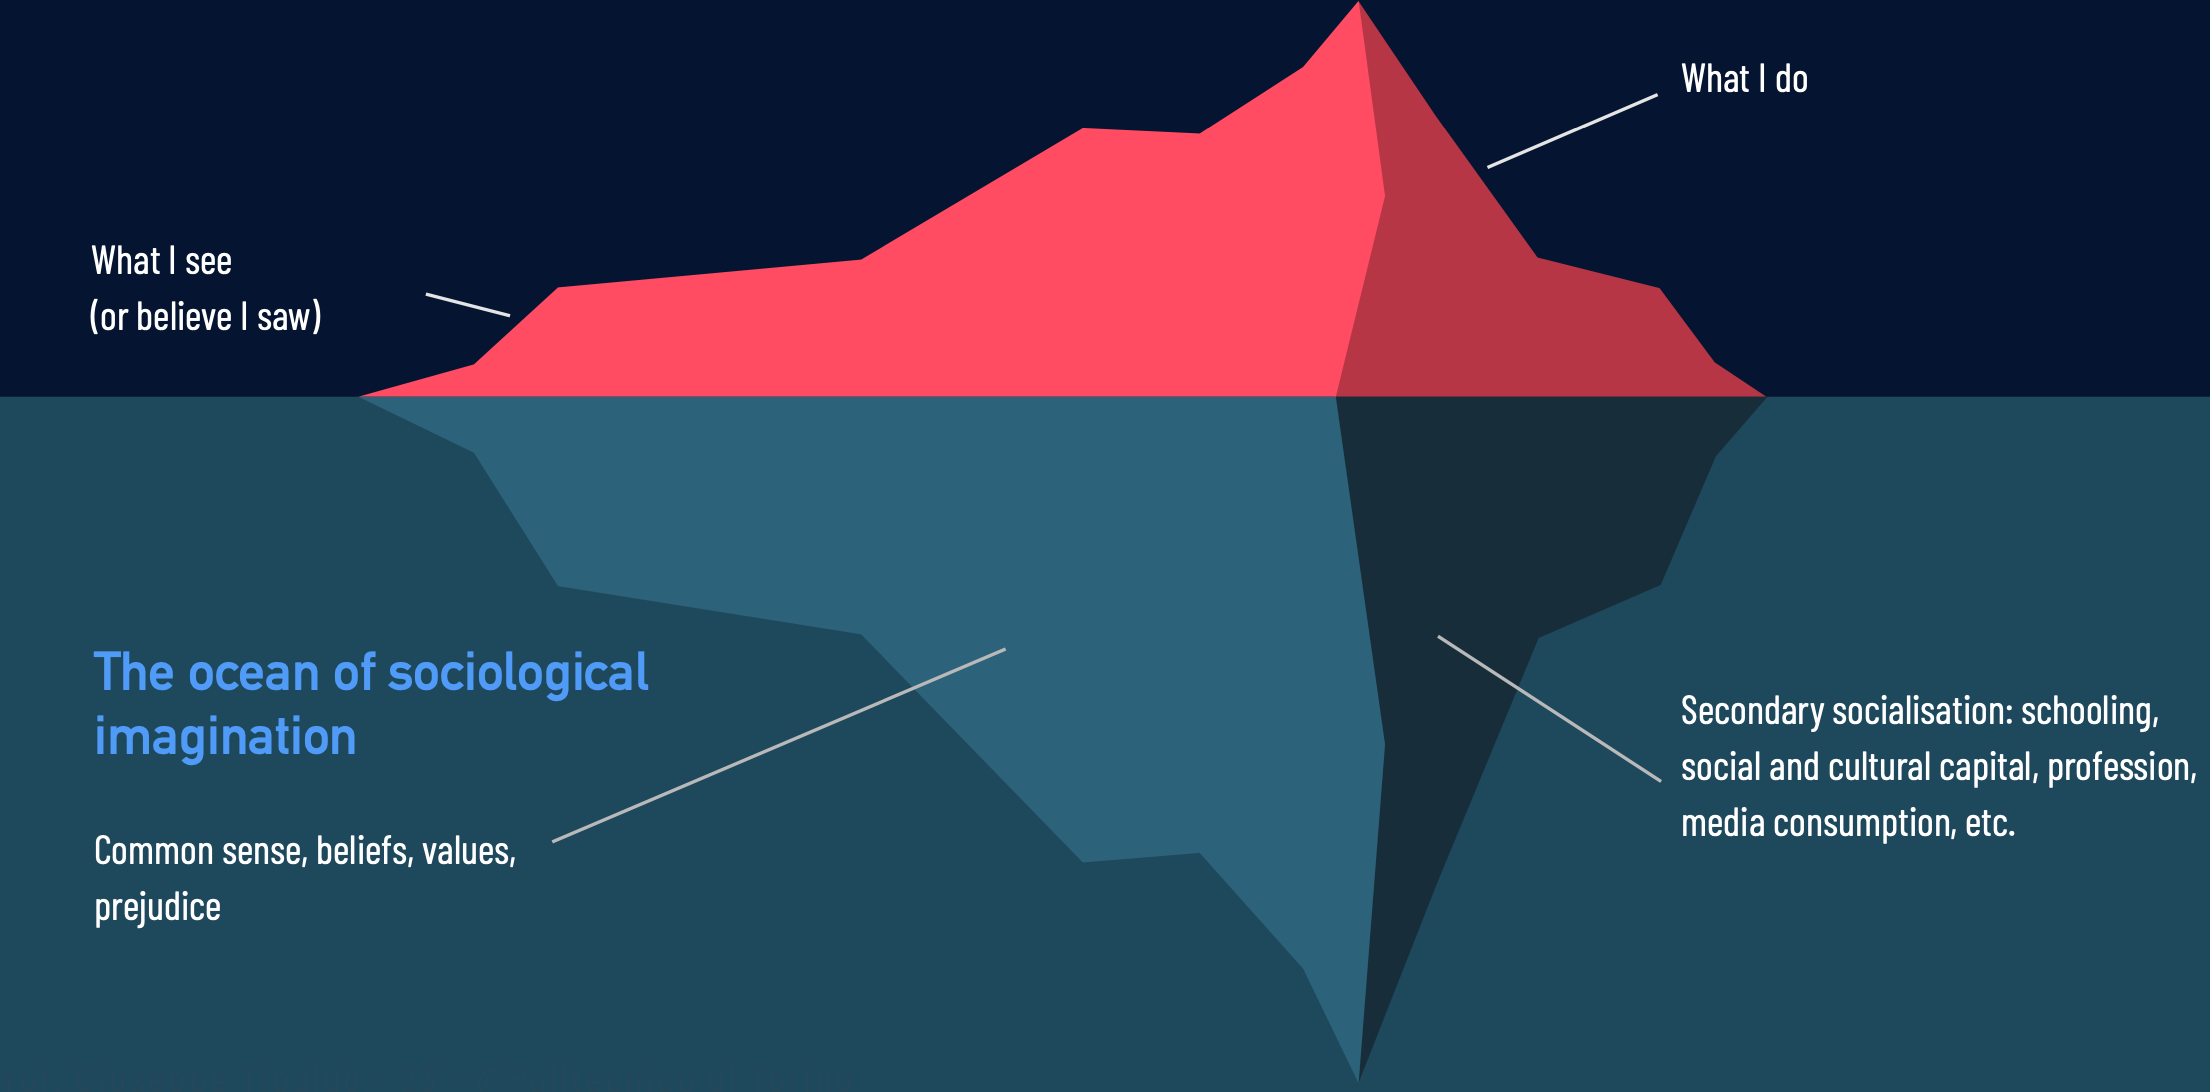
\includegraphics[width=\linewidth]{Images/Sociology/Iceberg.png}
    \caption{The Iceberg Relation}
    \label{fig:Sociology_Iceberg}
\end{figure}

\clearpage

\section{Nomina Nuda Tenemus}
“Nomina Nuda Tenemus” \footnote{This phrase is notably referenced in Umberto Eco’s The Name of the Rose, where it highlights the importance of meaning beyond mere names.} translates to “we hold only bare names.” It suggests that without deeper understanding or context, words are merely empty labels. 
Without a clear name or definition—in this case, within the realm of cybersecurity—it becomes impossible to identify what needs protection. Moreover, this lack of clarity prevents the formulation of an effective legal framework.
\subsection{Overview of Cybersecurity}
The diagram \ref{fig:Overview} provides an overview of cybersecurity from a sociological perspective, broken down into two main sections: Definitions and Terminologies and Concepts. Here's an explanation of each component:
\begin{itemize}
    \item Definitions: This section focuses on defining key concepts like cybercrime and cybersecurity. It includes an analysis of the historical development of these fields and discusses current trends in cyber threats and protection strategies.
    \item Terminologies and Concepts: This section introduces foundational terms necessary for understanding cybersecurity, such as malware, phishing, and ransomware. It highlights the necessity of a shared vocabulary for precisely identifying and describing cyber threats, offering structured classifications and comprehensive definitions of cybercrime.
\end{itemize}

\begin{figure}[H]
    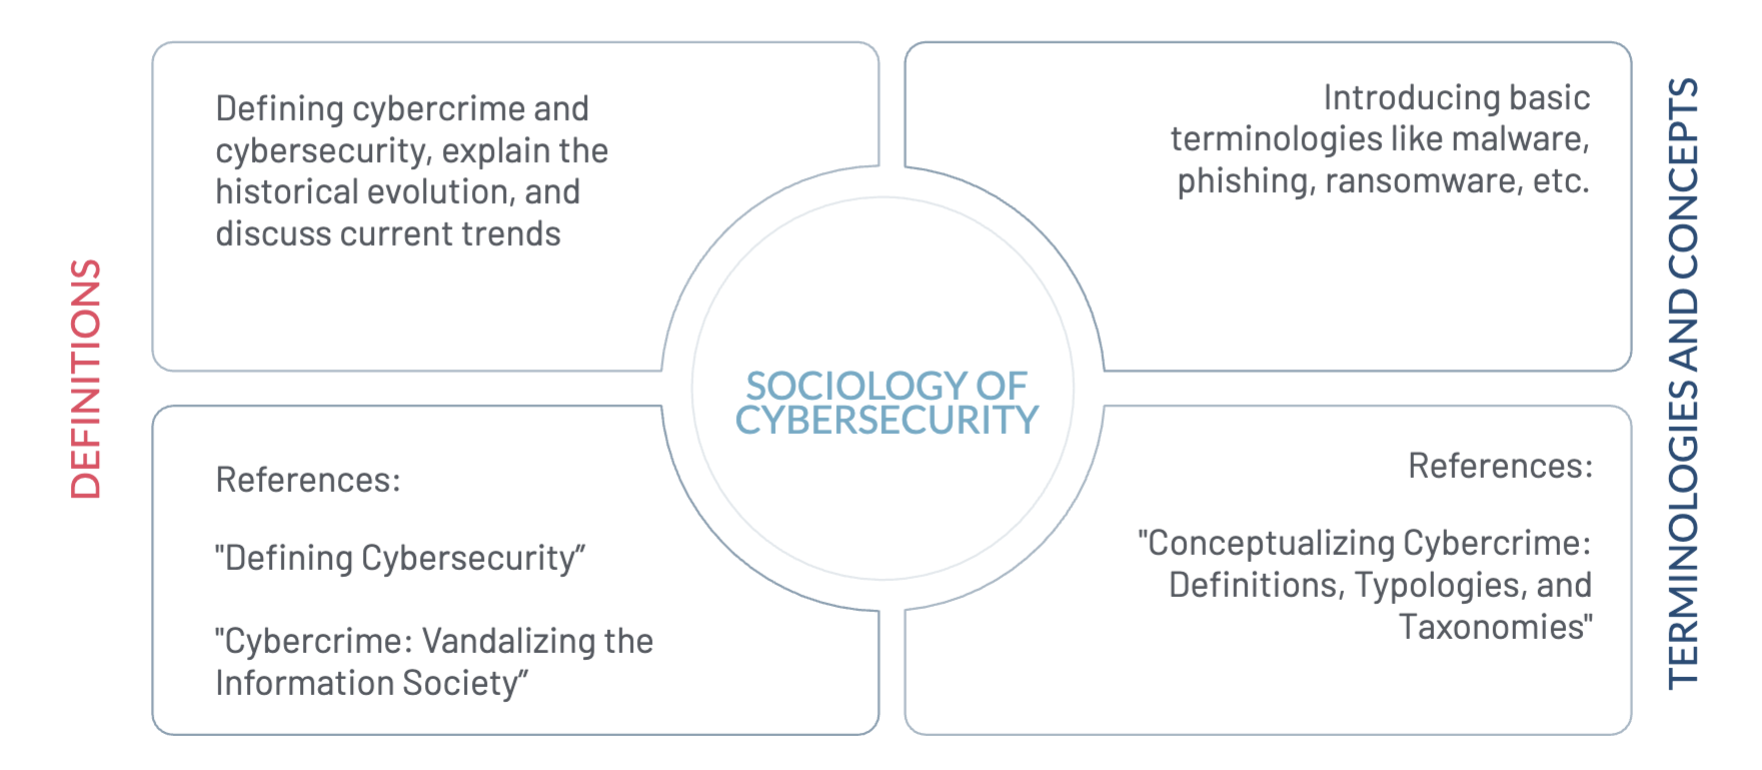
\includegraphics[width=\linewidth]{Images/Sociology/Overview.png}
    \caption{Overview of Cybersecurity from a sociological perspective}
    \label{fig:Overview}
\end{figure}

\subsection{Definitions of Cybercrime}
\subsubsection{Vocabulary}
Figure \ref{fig:Vocabulary1} illustrates how the vocabulary used to describe similar phenomena has changed over time. Nowadays, cybercrime attacks are a top priority on the agenda of many countries.
\begin{figure}[H]
    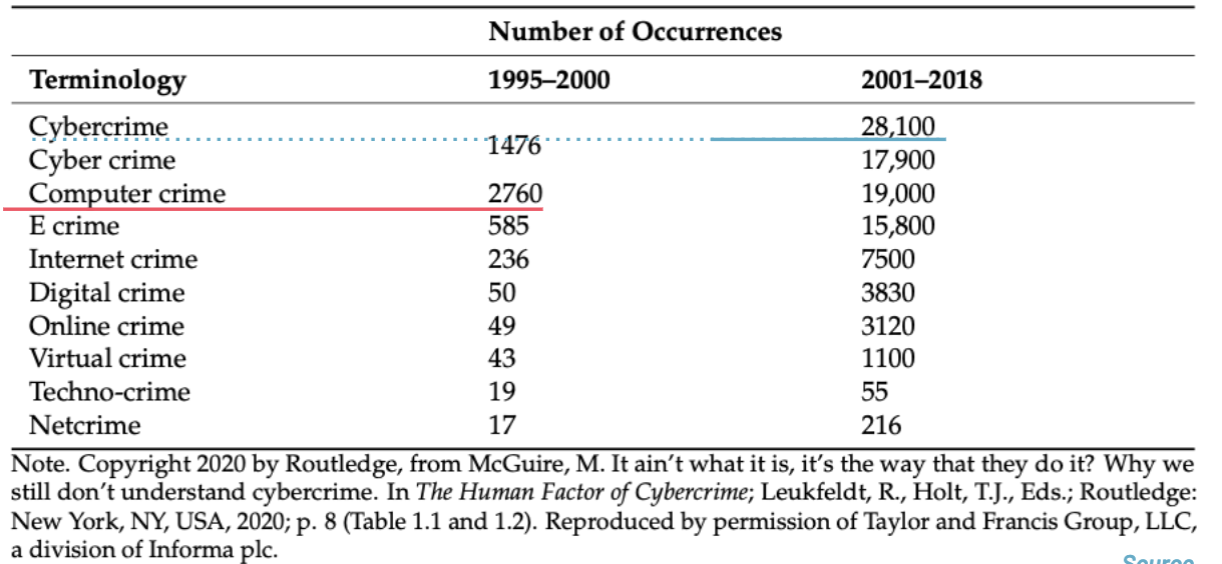
\includegraphics[width=\linewidth]{Images/Sociology/Vocabulary1.png}
    \caption{Cybercrime terminology in the periods 1995-2000 and 2001-2018}
    \label{fig:Vocabulary1}
\end{figure}

\subsubsection{Official Definitions}
Figure \ref{fig:Definitions} illustrates a shift from material to immaterial concerns regarding cybercrime attacks. In 1994, the United Nations issued the first official document, although cybercrimes already existed at that time, even if they were not yet formally named. Initially, cybercrimes were strictly related to the computer sphere. Over time, however, the definition of cybercrime expanded to encompass a broader range of activities, incorporating various new aspects. The main points of the new definitions are: data processed by computer systems or networks and information systems, either as a primary tool or as a primary target.

\begin{figure}[H]
    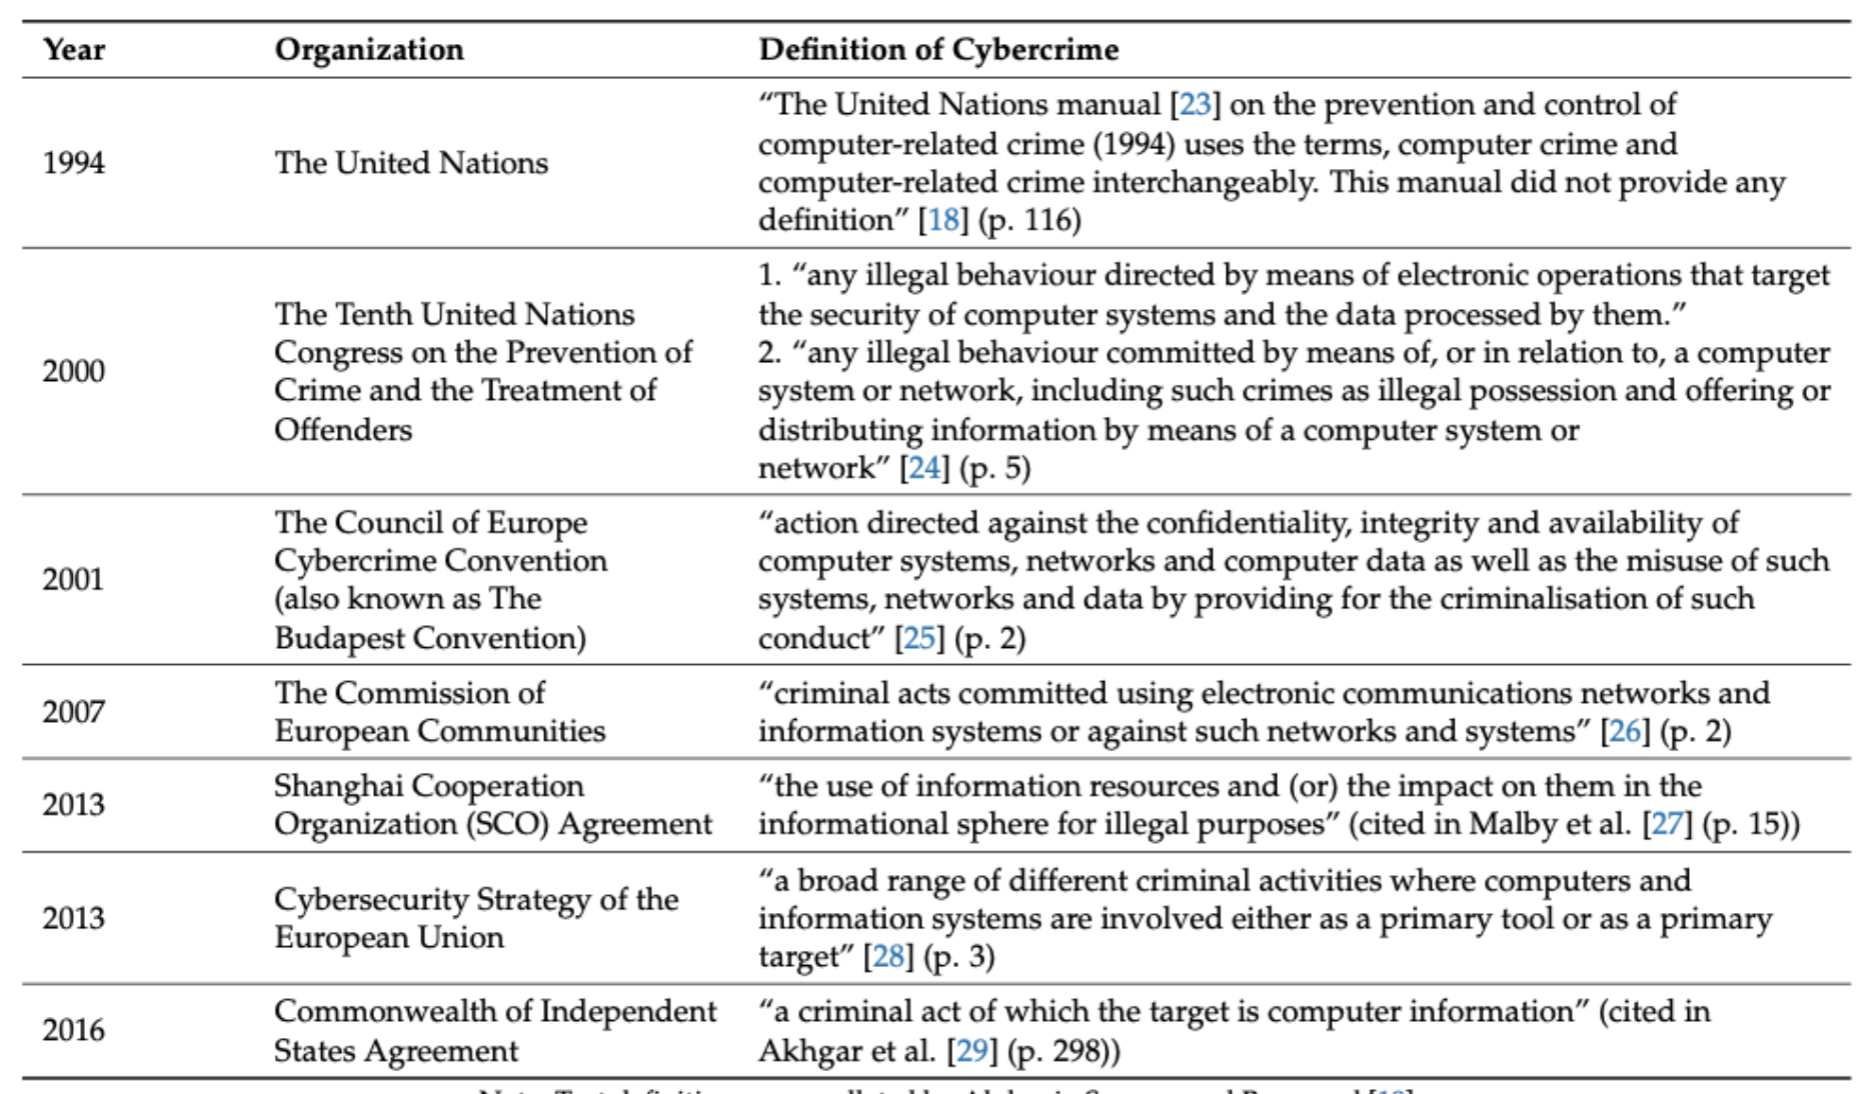
\includegraphics[width=\linewidth]{Images/Sociology/Definitions.png}
    \caption{Organization definitions of cybercrime}
    \label{fig:Definitions}
\end{figure}

\subsubsection{Dichotomous Definitions}
\begin{multicols}{2}
    In research and policymaking, a distinct dichotomy was established. A discrete categorical approach was applied to define cybercrimes, classifying them as either cyber-enabled or cyber-dependent. Cyber-enabled crimes are traditional offenses that predate the advent of technology but are now facilitated or made easier (i.e., enabled) by digital technology. Cyber-dependent crimes are crimes that arose with the advent of technology and cannot exist (i.e., dependent) outside the digital world. 
    \columnbreak

    Many people also agree with another, non-discrete dichotomy from a continuum approach perspective. The continuum approach to cybercrimes views cybercrime not as a discrete category but as a spectrum, where offenses range from traditional crimes that are cyber-enabled to those that are fully cyber-dependent. Crimes of Type 1 are more technical in nature, while crimes of Type 2 involve more human interaction.

\end{multicols}

\begin{multicols}{2}
    \begin{figure}[H]
        
\includegraphics[width=\linewidth]{Images/Sociology/CategoricalApproach.png}
        \caption{Categorical approach to cybercrime}
    \end{figure}
    \columnbreak
    
    \begin{figure}[H]
        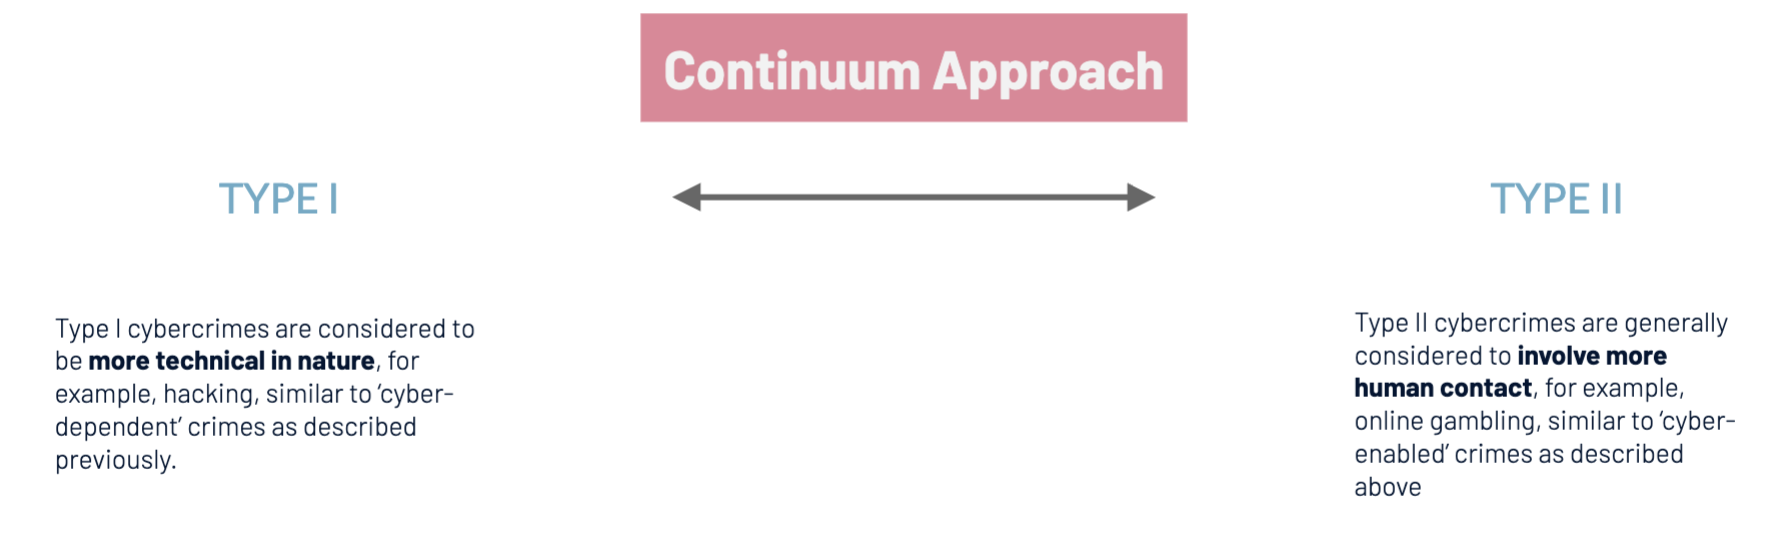
\includegraphics[width=\linewidth]{Images/Sociology/ContinuumApproach.png}
        \caption{Continuum approach to cybercrime}
    \end{figure}

\end{multicols}

\subsubsection{Trichotomous Definitions}
Industries have also attempted to classify clusters of crimes using trichotomous definitions within a categorical approach. First, we analyze the one made by David S. Wall in 2007. Wall introduced three sections:
\begin{itemize}
    \item Crimes against the machine: Computer integrity crimes (e.g., hacking).
    \item Crimes in the machine: known as computer content crimes (e.g., online hate).
    \item Crimes using the machine: Computer-assisted crimes (e.g. piracy).
\end{itemize}
The EU Commission also released labels in 2013 addressing cybercrimes, which share many similarities with the ones presented above. In fact, cybercrimes were divided in three stages: offenses unique to computers and information systems, content-related offenses and traditional offenses.

\subsection{Cybersecurity is}

As stated by Fredrick Chang, former Director of Research at the National Security Agency in the United States:
\begin{quotation}
    A science of cybersecurity offers many opportunities for advances based on a \textbf{multidisciplinary approach}\footnote{Crimes concern many fields of phenomena.}, because, after all, cybersecurity is fundamentally about an \textbf{adversarial engagement}. Humans must defend machines that are attacked by other humans using machines. So, in addition to the critical traditional fields of computer science, electrical engineering, and mathematics, perspectives from other fields are needed.
\end{quotation}

Analyzing literature\footnote{Craigen et al.2014} "Cyber" is a prefix connoting cyberspace and refers to electronic communication networks and virtual reality.
The term "cyberspace" describes a vision of a three-dimensional space of pure information, moving between computer and computer clusters where people are generators and users of the information. Public Safety Canada\footnote{2010} defines cyberspace as "the electronic world created by interconnected networks of information technology and the information on those networks. It is a global common where people are linked together to exchange ideas, services, and friendships."

